\section{Appendix}
\appendix
\subsection{Effects of priors on $n'(r)$}
\begin{figure*}
  \begin{center}
    \hspace{-7mm}
    \includegraphics[width=0.3\textwidth]{fig/Gaia07_nr_bound/output/pdf/prof_nr_0.pdf}
    \includegraphics[width=0.3\textwidth]{fig/Gaia07_nr_bound/output/pdf/prof_rho_0.pdf}
    \includegraphics[width=0.3\textwidth]{fig/Gaia07_nr_bound/output/pdf/prof_beta_1.pdf}
  \end{center}
  \begin{center}
    \includegraphics[width=0.3\textwidth]{fig/Gaia07_nr_free/output/pdf/prof_nr_0.pdf}
    \includegraphics[width=0.3\textwidth]{fig/Gaia07_nr_free/output/pdf/prof_rho_0.pdf}
    \includegraphics[width=0.3\textwidth]{fig/Gaia07_nr_free/output/pdf/prof_beta_1.pdf}
  \end{center}
  \begin{center}
    \caption{Influence of $dn(r)/d\log r$ prior. The top panels show
      $n(r)$, $\rho(r)$, and $\beta^*(r)$ for Gaia07 with a moderate
      prior of $|dn(r)/d\log r|<1.5/(8/N_{\rm ipol})$, the lower
      panels show the same profiles with two times this value. We see
      that a tighter prior on $n(r)$ yields tighter constraints on $\beta^*$.}
    \label{fig:nrprime}
    \end{center}
\end{figure*}



\subsection{Convergence of the \MultiNest\ model ensemble}
We check the convergence of the MCMC twofold: first, the range of
density profiles swept after 3k, 30k, 300k, and 3000k stays
approximately constant after 300k iterations, and gives us confidence
that we found and fully explored the valid regions of phase space in
density. See fig. ~\ref{fig:convergencedens}.

\begin{figure*}
    \begin{center}
        \hspace{-7mm}
        \includegraphics[width=0.25\textwidth]{fig/Walk02_3e3models/output/pdf/prof_rho_0.pdf}
        \includegraphics[width=0.25\textwidth]{fig/Walk02_3e4models/output/pdf/prof_rho_0.pdf}
        \includegraphics[width=0.25\textwidth]{fig/Walk02_3e5models/output/pdf/prof_rho_0.pdf}
        \includegraphics[width=0.25\textwidth]{fig/Walk02_3e6models/output/pdf/prof_rho_0.pdf}
        \caption{Density profile of the Walk02 model after
          (3k,30k,300k,3000k) iterations (left to right). There is no
          signifikant change of the $2\sigma$ area swept by the models
        after 300k iterations.}
        \label{fig:convergencedens}
    \end{center}
\end{figure*}

Second, the range of $\beta_i$, the other unrestricted parameters, show
a similar behaviour, as shown in ~\ref{fig:convergencebeta1} for $\beta_1$,
with analogous $\beta_2$.

\begin{figure*}
   \begin{center}
       \hspace{-7mm}
       \includegraphics[width=0.25\textwidth]{fig/Walk02_3e3models/output/pdf/prof_beta_1.pdf}
       \includegraphics[width=0.25\textwidth]{fig/Walk02_3e4models/output/pdf/prof_beta_1.pdf}
       \includegraphics[width=0.25\textwidth]{fig/Walk02_3e5models/output/pdf/prof_beta_1.pdf}
       \includegraphics[width=0.25\textwidth]{fig/Walk02_3e6models/output/pdf/prof_beta_1.pdf}
       \caption{Convergence of $\beta_1$ after (3k, 30k, 300k, 3000k) iterations (left to right).}
       \label{fig:convergencebeta1}
   \end{center}
\end{figure*}


\subsection{The choice of binning}
\TODO{Consider the effect of varying the number of particles per bin for a single model.}
\TODO{explore different binning and lower sampling in an appendix}

%%% Local Variables:
%%% mode: latex
%%% TeX-master: "Steger_2014_GravImage"
%%% End:
